\section{Ensemble Selection}
\label{ES}
Any supervised predictive model makes an assumption on the distribution underlying the data $x$ and uses this approximation to the true distribution to infer from training data to predict the labels $y$ of new data. During the training of the model, a trade-off between fit and generalization has to be considered. A classifier might be able to fit training data perfectly but fail to generalize to new data and vice versa. 
 
One way of mitigating this issue is the construction of an ensemble which is ``a set of classifiers whose individual decisions are combined in some way (typically by weighted or unweighted voting) to classify new examples." \cite[p. 1]{dietterich2000ensemble} There are three main explanations as to why model ensembles tend to perform better than single classifiers: the first (\emph{statistical}) reason the weighting of classifiers averages different assumptions on the data and therefore approximates the true data generating function better than a single assumption could. The second (\emph{computational}) reason is that single classifiers tend to find local optima and combining their predictions has a higher potential of approximating the global optimum. The third (\emph{representational}) reason asserts that not all types of classifiers are able to represent the true data generating process or at least cannot consider all representations in a finite sample \cite[p. 2--3]{dietterich2000ensemble}. %Besides these theoretical assumptions on the performance of ensembles, there are numerous empirical studies to show that the combination of multiple even weak classifiers can yield a strong ensemble classifier.

Following the notation by \cite{tsoumakas2008taxonomy}, the problem of Ensemble Selection (ES) can be represented as follows: let $x$ be realizations of $X$ and let $h_i, i=1,\dots,k$ be a set of base classifiers that return probabilities $m_i(x, c_j)$ for $j = 1,\dots,d$ for each label $c_j$. The ensemble then outputs:
\begin{equation}
y(x) = \text{arg max} \sum_{i=1}^{k} w_i m_i(x,c_j),
\end{equation}
where $w_i$ is the weight for classifier $m_i$. One seeks to optimize $w$ such that the predictions are as accurate as possible \cite[p. 2]{tsoumakas2008taxonomy}.

ES relies on two key assumptions: the single classifiers have to be 1. accurate and 2. diverse. Accuracy means that the classifier has be at least better than a random guess. Diversity means that the single classifiers have different decision boundaries, i.e. produce different predictions. Diversity among the classifiers helps achieve the averaging of different types of errors \citep{brown2005diversity}. An idealized visualization of this assumption can be seen in Figure \ref{fig:diversity}. So far, there is no canonical definition of diversity and one can choose between a number of different measures. The question of whether more diverse ensembles always produce better predictions cannot be answered with certainty as the empirical results are not straightforward \cite[p. 203]{Kuncheva2003}. For an extensive overview see \cite{Kuncheva2003} and \cite{kuncheva2005using}.
\begin{figure}
	\centering
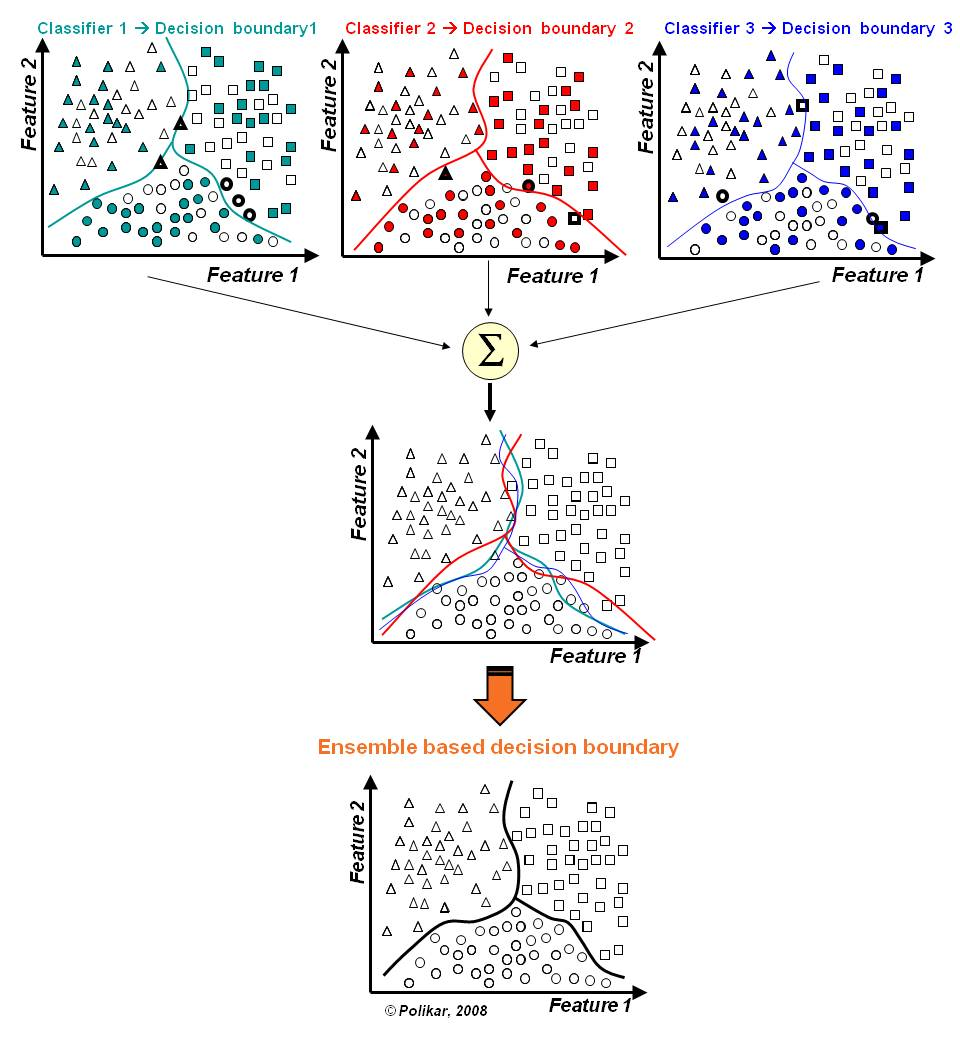
\includegraphics[scale=0.35]{Combining_classifiers2}
\caption{The combination of classifiers with different decision boundaries improves predictive power \citep{polikarphoto}.}
\label{fig:diversity}
\end{figure}

Bagging, \textbf{B}ootstrap \textbf{agg}regat\textbf{ing}, originally refers to the training of classifiers of one type on random resamples of the training data \citep{Breiman1996}. For the training of $k$ classifiers, $k$ training sets of size $N$ are generated by drawing from the original data set of size $N$ with replacement. While the individual classifiers' errors on the test set increase with that technique due to overfitting to the samples that occur more often in the training set, the combination of these overfitted classifiers makes the ensemble so strong \cite{krogh1996learning}.

An alternative to Bagging is Boosting where in a sequence of classifiers, incorrectly classified samples are resampled more often to improve the accuracy of the single classifier \cite[p. 173]{opitz1999popular}. Since 1996 both Bagging and Boosting have been expanded and applied at different steps of the classifier learning and final ES. Opitz and Maclin show that combining different classifiers that are trained on the same data, too, produces very good results \cite[p. 170]{opitz1999popular}. \\

One potential issue in ES is overfitting, i.e. the inclusion of many classifiers in the ensemble may produce good results on the training set but result in poor performance on the test set \cite[p. 253]{sun2011bagging}, \cite[p. 2092]{cawley2010over}. To prevent this, \cite{caruana2004ensemble} present a novel approach. They extend the simple iterative inclusion or exclusion of classifiers to an ensemble in three ways: 
\begin{description}
	\item[Selection with Replacement] Classifiers can be included in the ensemble several times meaning that good classifiers can be picked again instead of poorer ones when the initial top $t$ models have already been selected.
	\item[Sorted Ensemble Initialization] Instead of filling an empty ensemble, the initial ensemble is already comprised of the $t$ best classifiers and filled from there on.	
	\item[Bagged ES] In this case, instead of bagging the training data, subsets of classifiers are created. One then optimizes the classifier combination within the subset and results across all subsets are averaged to obtain the final ensemble.
\end{description}
As a demonstration of bagged ES, imagine that one draws 15 samples from a classifier library of 1000 with a probability $p =0.5$ such that each sample or bag contains 500 classifiers whose combination is then optimized with, for example, forward-selection. The 15 obtained sub-ensembles are then combined \cite[p. 3]{caruana2004ensemble}.
The empirical results of Caruana et al. point strongly towards setting the ratio of models per bag to 0.5 as it shows the strongest advantage over the baseline best model. They also show that ensemble selection works extremely well with any type of performance metric, \mbox{i.e. }accuracy, ROC, root mean-squared error, \mbox{etc. }and accounted for one third of the total 8.7\% outperformance of ES over the best model alone. Caruana et al. optimized the ES with forward stepwise selection where one iteratively adds classifiers until the performance converges. However, any selection or optimization procedure is possible. Linear methods include taking the simple average, the weighted average, or the median. Voting covers majority voting, plurality voting for multi-class problems, or weighted voting. For a more detailed view on ensemble combination see Chapter 4 in \cite{zhou2012ensemble}. Usually, the classifiers are combined with regards to some objective function, the ensemble accuracy for example. 

The problem of optimizing the classifier combination with regards to some objective function is a non-linear problem. A possible search heuristic for finding the optimal classifier combination are Evolutionary Algorithms, a class of algorithms that emulate different behavior found in nature: the evolution of genes or individuals over time or the movement of swarms or flocks. EAs solve the initial questions of which models to include and how to combine them heuristically and have shown competitive results in the past \citep{oliveira2005multi}.


%Probably add here: 'Overfitting cautious selection of classifier ensembles with genetic algorithms' by Santos:
%' However, even though the control of overfitting is a challenge in machine learning problems, much less work has been devoted to the control of overfitting in selection tasks. The objectives of this paper are: (1) to show that overfitting can be detected at the selection stage; and (2) to present strategies to control overfitting. Decision trees and k nearest neighbors classifiers are used to create homogeneous ensembles, while single- and multi-objective genetic algorithms are employed as search algorithms at the selection stage. In this study, we use bagging and random subspace methods for ensemble generation. The classification error rate and a set of diversity measures are applied as search criteria. We show experimentally that the selection of classifier ensembles conducted by genetic algorithms is prone to overfitting, especially in the multi-objective case. In this study, the partial validation, backwarding and global validation strategies are tailored for classifier ensemble selection problem and compared.'


